%----------------------------------------------------------------------------------------
%	PACKAGES AND DOCUMENT CONFIGURATIONS
%----------------------------------------------------------------------------------------

\documentclass[
	letterpaper, % Paper size, specify a4paper (A4) or letterpaper (US letter)
	10pt, % Default font size, specify 10pt, 11pt or 12pt
]{class}

\usepackage{caption}
\usepackage{soul}
\usepackage{subcaption}

\addbibresource{bibliography.bib} % Bibliography file (located in the same folder as the template)

%----------------------------------------------------------------------------------------
%	REPORT INFORMATION
%----------------------------------------------------------------------------------------

\title{Airline Departure\\Data Analysis and Regression} % Report title

\author{Lucchi Manuele \& Tricella Davide} % Author name(s), add additional authors like: '\& James \textsc{Smith}'

\date{\today} % Date of the report

%----------------------------------------------------------------------------------------

\begin{document}

\maketitle % Insert the title, author and date using the information specified above

\begin{center}
    \begin{tabular}{l r}
        Instructors: Professor \textsc{Cesa-Bianchi} \& Professor \textsc{Malchiodi}
    \end{tabular}
\end{center}

%----------------------------------------------------------------------------------------
%	DECLARATION
%----------------------------------------------------------------------------------------

\textit{We declare that this material,
    which we now submit for assessment, is entirely our own work and has not been
    taken from the work of others, save and to the extent that such work has been cited and
    acknowledged within the text of our work. We understand that plagiarism, collusion,
    and copying are grave and serious offences in the university and accept the penalties that
    would be imposed should I engage in plagiarism, collusion or copying. This assignment,
    or any part of it, has not been previously submitted by us or any other person for
    assessment on this or any other course of study.}

%----------------------------------------------------------------------------------------
%	ABSTRACT
%----------------------------------------------------------------------------------------

\begin{abstract}
    The purpose of this paper is to evaluate the usage of a Logistic Regression model on a airlines dataset to predict flight cancellation or diversion, in a scalable and time/space efficient implementation.
\end{abstract}

%----------------------------------------------------------------------------------------
%	TOC
%----------------------------------------------------------------------------------------

\tableofcontents

%----------------------------------------------------------------------------------------
%	DEFINITIONS
%----------------------------------------------------------------------------------------

\section{Definitions}\label{definitions} % Labels provide a point for referencing, in this case with \ref{definitions} to refer to this subsection number

\begin{description}
    \item[Dataset] The sample of data used to train the Model
    \item[Label] The expected outcome of the prediction
    \item[Model] The group of algorithms that tries to solve the problem
    \item[Overfitting] When the model is too sensible to changes compared to the dataset
    \item[Vanishing Gradient] When the gradient values becomes progressively smaller until they are insignificant for the process
\end{description}

%----------------------------------------------------------------------------------------
%	INTRODUCTION
%----------------------------------------------------------------------------------------

\section{Introduction}

The paper is splitted in a describing part, where the operations on the dataset and how the model is built are detailed, and an experimental part where a series of tests are performed and the results are stated.\\

Also, the document covers two different objectives, the classification of the dataset using the model to predict both the \textbf{canceled} and the \textbf{diverted} flights.\\
The two objectives are virtually the same, since the subset of the dataset used is identical and the model stays the same.\\

Both the cases represent real world problems that are still not completely solved, since there aren't algorithms that predicts these situations with accuracy yet, so a simple Logistic Regression model is probably not powerful enough to accomplish this tasks, but it's still worth analyzing its behavior in different circumstances.

%----------------------------------------------------------------------------------------
%	DATASET
%----------------------------------------------------------------------------------------

\section{Dataset}

The initial dataset, "Airline Delay and Cancellation Data" \cite{dataset} is made of 9 years of airlines flights data, composed by 10 files (one for each year from 2009 to 2018) with around 6 milions records each.
The files presents 28 columns, of which only the 9 more relevant were took\\

\begin{description}
    \item[FL\_DATE] The flight date.
    \item[OP\_CARRIER] The carrier code.
    \item[ORIGIN] The departure airport.
    \item[DEST] The destination airport.
    \item[CRS\_DEP\_TIME] The planned departure time.
    \item[CRS\_ARR\_TIME] The planned arrival time.
    \item[CANCELLED] If the flight has been canceled.
    \item[DIVERTED] If the flight has been diverted.
    \item[CRS\_ELAPSED\_TIME] The planned total time of the flight, taxi time included.
    \item[DISTANCE] The distance the flight has to cover.\\
\end{description}

The majority of columns have been excluded because contained information not available at departure time, like the ones regarding actual departure, flight and arrival time, which are at disposal only after the aircraft landed.
Other columns also contained informations which do not have any correlation with the objective of the experiments, like the flight number assigned by the carrier.\\

In the case the prediction is about the cancellation, the \texttt{DIVERTED} column will be ignored, while if the prediction is on if the flight would be diverted or not, the \texttt{CANCELLED} column will be ignored.\\

The carrier code is a two characters alphanumeric code, the origin and destination places are a three characters alphanumeric code.\\
Flight date, departure time and arrival time are dates, while the elapsed time and the distance are real numbers.\\
Cancelled and diverted are either 0 or 1.\\

100,000 records sampled with an uniform distributed were took from each year file to perform the preprocessing. This number is due to the limited memory
possessed by the machine on which the tests have been performed.

%----------------------------------------------------------------------------------------
%	PREPROCESSING
%----------------------------------------------------------------------------------------

\section{Preprocessing Techniques}

\subsection{Null values removal}

Multiple preprocessing techniques were used.\\

The first operation consisted in the removal of the rows with null values, after counting them we concluded that the null values are really rare in the dataset, so it was possible to remove the rows entirely, without any significant loss of informations.\\

\subsection{Data Analysis}
After the null rows removal, some analysys have been performe using the charts of the MatPlotLib library, especially the bar charts.\\
The main objective of this analysis was to find an eventual correlation between the various features used and the probability that a flight would be cancelled dor diverted.\\

Unfortunately, none of the features showed significative patterns nor tendencies of the problematic flights to increase in relation to a particular value of a feature or a combination of features.\\

\subsubsection{Problematic flights per carrier}
The first chart we draw tried to correlate the carriers with an abnormal number of the cancelled flights, to make the chart more readable, we aggregated in one column every carrier with a percentage lower than the mean of all carriers, to show only the highest percentages.\\

The result was a chart showing some carriers with a slightly-above-average number of cancelled flights, and a peak of 4\% of the flights  cancelled, but considering the huge number of distinct carriers in the dataset, the impact of this feature will probably be very low.

\begin{center}
    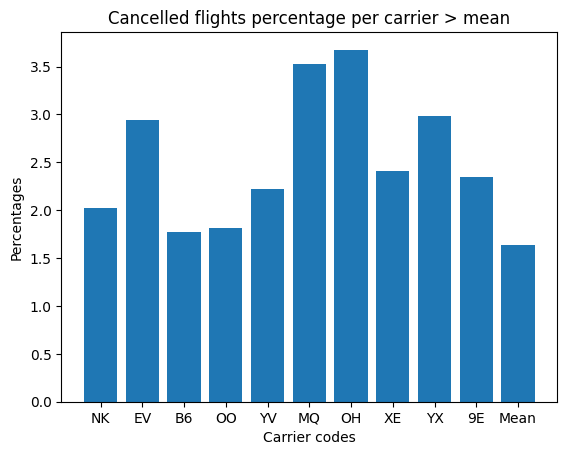
\includegraphics[width=10cm]{../images/cancelled_per_carrier.png}
\end{center}

\subsubsection{Problematics flights per origin}
The second analysis was performed on the origin feature.
The first chart plotted was a box plot, because due to the high number of airports, the bar was overcrowded and diffcult to read.\\

The result can be considered an improvement regarding the correlation between a feature and the result, because thre are some origins that posses a significant percentage
of problematic flights, with a peak of over 25\% of cancelled flights. This cannot be taken as a decisive factor though, because while the probability of those particular airports increase notably, the vast majoerity of the origins (at least two quartiles), show no evident correlation with this feature.

\begin{center}
    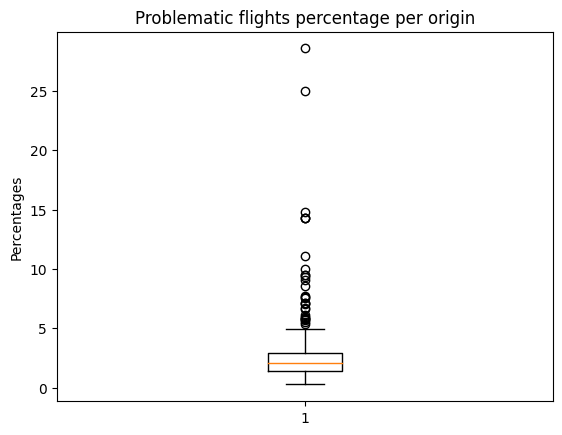
\includegraphics[width=10cm]{../images/cancelled_box_per_origin.png}
\end{center}

To show a readable bar chart, the same technique as before has been applied, aggregating the values of the majority of origins inside one column. This time though it was not enough to aggregate columns aunder the mean of the values, so we used a fixed number to aggregate, which is switched based on the problem to solve,
because the diverted problem posesses lower percentages of problematic flights.

\begin{center}
    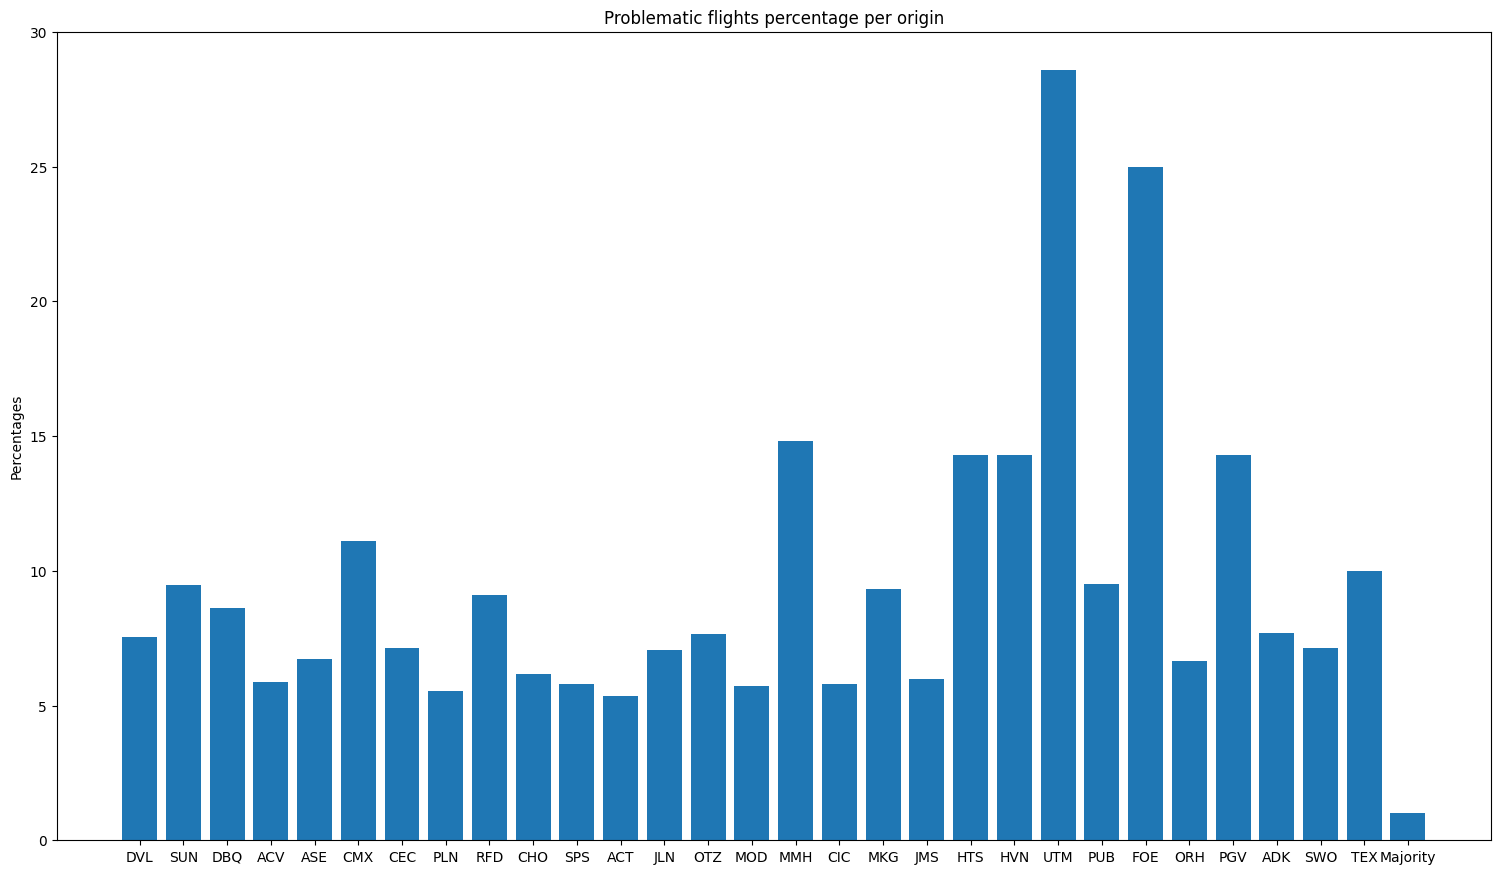
\includegraphics[width=14cm]{../images/cancelled_per_origin.png}
\end{center}
\newpage

\subsubsection{Problematics flights per month}
Trying to find a correlation between the year period and the problematic flights, we plotted a chart based on the month of the flight. The result was expectedly skewed towards the winter months, where the bad weather conditions can influence the flight departures, but even in this case, the difference was not so dramatic, always remaining in a few percentage points.

\begin{center}
    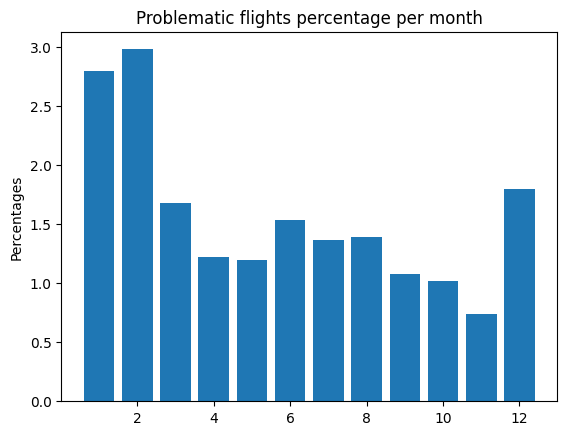
\includegraphics[width=10cm]{../images/cancelled_per_month.png}
\end{center}

\subsubsection{Problematics flights per weekday}

The last chart we plotted was based on the weekday of the flight, trying to see if there was a relation between particular days and the rise of problematic flights.\\

Unfortunately this was the more useless analysys performed, with every column of the chart being almost identical to each other, basically this information doesn't tell anything about the probability of a flight of being problematic or regular.

\begin{center}
    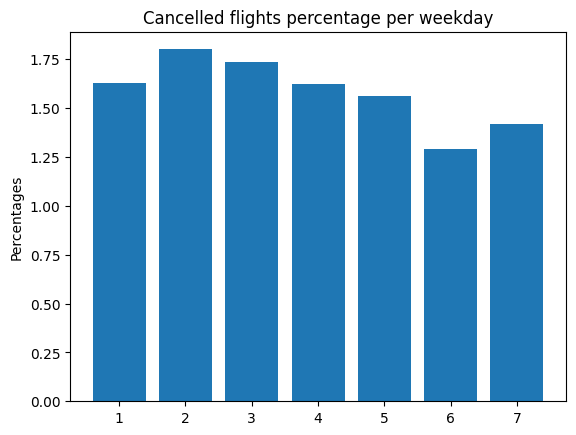
\includegraphics[width=10cm]{../images/cancelled_per_weekday.png}
\end{center}

\subsection{Data conversions}

All the data not already represented as real numbers has been converted; airports and carriers identifiers, that were alphanumeric codes, had a number assigned based on the code. Dates were splitted between the year and the rest, the former has been discarded, while the latter has been hashed.\\

\subsubsection{Hashing}

Particularly, to convert the identifiers, the checksum function \textbf{crc32} \cite{crc32} has been used, then the result has been put in END with the bytes representing the number -1, to ensure to get an unsigned integer. Finally, the value is normalized dividing it for the max integer value.
This function has been chosen because is one of the fastest way to hash short strings, which is what is needed here, compared to other alghoritims like the SHA or MD5.\\

\subsubsection{Normalization}

To normalize dates, the day of the year has been extracted from every date, then divided by 365. A similar strategy has been used for the departure and arrival times, exctracting the minutes of the day and then dividing by 1140.\\

The distance has been normalized by dividing it for the maximum value found in the dataset, rounded by excess to 4970.\\

At this point, the dataset has been balanced in regard of the evaluated property, be it being canceled or diverted, so that there are an equal number of uniformly drawn positives and negatives.\\

The converted values were also limited between 0 and 1, to avoid exploding values during the training of the dataset.\\

\subsubsection{Balancing}

This was necessary since the diverted or cancelled flights are a really small percentage of the overall flights,
this in the first tests has been proved to be a problem, because the trained model always responded that no flight would have been cancelled or diverted, since it has been trained on a dataset with basically zero problematic flights.\\

To solve the problem, we used the \textbf{Undersampling} technique, matching the number of normal flights and problematic flights, limiting the amount of normal flights that has been kept.\\

Since less than 0.1\% of the dataset are positive cases (for both the tasks) after the oversampling, the recordsa remained are just some tens of thousands, instead of hundreds of thousands, half with positive outcomes and half with negative ones.

\subsubsection{Z-Score Normalization}
Before the actual computation, the dataset has been normalized again by subtracting the \textbf{mean} and dividing by the \textbf{standard deviation}. This is called \textbf{Standard Score} \cite{normalization} or Z-Score Normalization.\\

The purpose of this normalization is to present to the model data that possesses less noise, improving the training performance. Particularly in this scenario, where the model proposed is simple and not sophisticated enough to work well with data that are not normalized.

\subsubsection{K Fold Cross Validation}
After the dataset has been processed, the resulting data must be splitted into a \textbf{training} part and a \textbf{testing} part. To avoid bias towards specific parts of the dataset, the K-Fold Cross Validation \cite{crossvalidation} was used.\\

This technique consists on splitting the dataset into K equally distributed and sized parts called folds, and while K-1 folds will be used for the training, the other one will be used for testing. This process will be repeated for K time, using each time a differend fold for the testing (and consequently excluding it from the training)\\

During the split, the percentages of positives and negatives cases have been kept costant for every partition, we also ensured that every fold has a different set of rows to avoid overlapping of any kind.

$$ x' = \frac{x - \mu}{\sigma} $$

\subsection{Parallelization}

\subsubsection{PySpark}
Keeping in mind that the implementation has to be space and time efficient and \textbf{scale up to large datasets}, the preprocessing part has been carried out using the library PySpark.
PySpark is a wrapper for Python of the library Apache Spark \cite{spark}, originally written in Java.\\

The purpose of this library is the handling of \textbf{parallelized data processing}, particularly regarding the Distributed File System Hadoop, also created by the Apache Foundation.
The library handles automatically the work distribution on the available nodes that the system provide, it can be composed of a single machine with multiple cores or a cluster of machines, this improves significantly the \textbf{scalability} of the solution, which can be run on competely different system without code modification.\\

\subsubsection{Compatibility}

The usage of this library created some compatibility issues, because the data structures used by PySpark were not compatible with various parts of the preprocessing section, which had been written initially using the data science library Pandas \cite{pandas}.\\

To solve these problems, it wasn't possible to simply use a conversion and leave the parts written in Pandas as they were, because the computation would have run on a single machine, without parallelization, making the use of PySpark completely pointless.
The issue has been addressed using the \textbf{PySpark.SQL} functionality, which allow to execute queries on a distributed dataframe. For our purposes various UDF (User Defined Functions), have been created, which then have been applied to every column containing certain types of data.
When it was possible, the conversions have been accomplished using a select method only, because the UDF functions are not as optimized as the native ones, making the computations with UDF significantly longer.\\

To evaluate the differences between the PySpark and Pandas performances, the preprocessing part has been implemented using both methods, with the possibility to test the Pandas implementation in its own code cell.

\subsubsection{I/O}

The library PySpark is also able to handle the csv file reading and writing, so it has been used to save the preprocessed data to speed up multiple runs on the dataset. To carry out the writing of the various distributed dataframes, various files are created, then at the time of reading, the data is distributed to the various nodes. There are two intermediate csv files, one for the 'cancelled' problem and one for the 'diverted' problem.\\

\subsubsection{Data structures}

The preprocessing part of the solution uses the PySpark \textbf{Dataframe} structure, the main reason for this choice is to take advantage of the column notation. This makes the code cleaner and easier to read, than the standard RDD (Resilient Distributed Dataset) implementation. The dataframe SQL functions are also really handy to convert efficienlty the various columns of the dataframes.
However, after the preprocessing, entering the training section of the project, we noticed that the RDD structure was better suited to accomplish the various calculations required by the model, so the folded dataframes were converted to RDDs before passing them to the next section.

%----------------------------------------------------------------------------------------
%	MODEL
%----------------------------------------------------------------------------------------

\section{Model}

The proposed model is a simple Logistic Regression \cite{logistic} algorithm that makes use of a few techniques to avoid overfitting (batching, L2 regularization) and uses the Gradient Descent as a solver.\\
The implementation uses \textbf{numpy} \cite{numpy} as its primary library of mathematical functions

\subsection{Parameters initialization}
Parameters such as Weights and Bias are initialized using a \textbf{uniform distribution} between 0 and 1, with the first one having the same length as the number of columns and the second being a scalar value.
The other hyperparameters were tuned throught various experiments that will be detailed later.

\subsection{Algorithm}

\subsubsection{Estimate}
The estimate is computed as follows
$$ \hat{y} = \sigma(w^Tx + b) $$
where $\sigma$ is the Sigmoid function \cite{sigmoid} and it's defined as
$$ \sigma(z) = \frac{1}{1 + e^{-z}} \in [0,1] $$
and $w$ and $b$ are the model weights and bias and $x$ is the input.

The code implementation uses \texttt{np.exp} for the exponential calculation.

\subsubsection{Gradient}

$$ \nabla w = \frac{1}{m}x^T(\hat{y} - y) $$
$$ \nabla b = \frac{1}{m}\sum(\hat{y} - y) b $$

In the code implementation, \texttt{np.dot} and \texttt{np.mean} were used.

\subsubsection{Update}

Gradient Descent \cite{sgd} is a technique that allows to find maximus e minimum in a multi-variable function, like the model taken in consideration.\\
Once the gradients are calculated, the parameters (weights and bias in this case) will be updated with the gradient value properly mitigated with the \textbf{Learning Rate}

$$ w' = w - \mu \nabla w $$
$$ b' = b - \mu \nabla b $$

\subsubsection{Loss}
For the loss the \textbf{Binary Cross Entropy} \cite{binarycrossentropy} function, also called \textbf{Log Loss}, was used.
It is defined as
$$ loss(\hat{y}, y) = -\frac{1}{n}(y log(\hat{y}) + (1-y)log(1-\hat{y})) $$
This particular function is used since, to perform the gradient descent, it can be derived and conducted to the weights update formula to minimize the loss in the same way as it's done for the MSE \cite{mse} in the Linear Regression.\\

For the MSE and Linear Regression

$$ MSE(w) = \frac{1}{2} (\hat{y} - y)^2 = \frac{1}{2} (w^Tx - y)^2 $$
$$\frac{\partial J}{\partial w} = (w^T x - y)x $$
$$ w' = w - \mu (w^T x -y)x $$

For the Log Loss and Logistic Regression

$$ LogLoss(\hat{y}, y) = -y log \hat{y} - (1-y)log(1- \hat{y})$$
$$ \hat{y} = sigmoid(w^Tx) = \frac{1}{1 + e^{w^Tx}} $$
$$ \frac{\partial LogLoss}{\partial w} = (\hat{y} - y)x $$
$$ w' = w - \mu (\hat{y} - y)x $$
$$ w' = w - \mu (w^T x -y)x $$

\subsubsection{Batching}
There are multiple types of Gradient Descent.\\

\textbf{Stochastic Gradient Descent} updates the model after each sample and has a convergence rate that is non-linear $O(\frac{1}{k})$ where $k$ is a fixed step size.\\

\textbf{Batching Gradient Descent} updates the model once per iteration using the whole dataset at once. It has a better convergence rate.\\

\textbf{Mini Batch Gradient Descent} \cite{batching} uses small chunks of samples, so it's a middle solution between the previous ones, but adds a new hyperparameter to tune, the \textbf{Batch Size}.\\
Its convergence rate is
$$O(\frac{1}{\sqrt{bk}} + \frac{1}{k})$$

In this project the last one was choosen after a dedicated experiment.

\subsubsection{Regularization}
Regularization is a technique used to prevent the overfittings. A regularization term is added to the optimization problem (i.e. the gradient calculation) to avoid overfitting.
The used version is called \textbf{L2}, also known as \textbf{Ridge Regression} \cite{l2}.\\

The regularization factor for the loss is defined as
$$ L2 = \frac{\lambda}{2}||w||^2 $$
where $L2$ is calculated as
$$ \frac{\lambda}{2}||w||^2 = \frac{\lambda}2{\displaystyle\sum_{j=1}^m w_j^2} $$ \\

The loss then becomes
$$ loss(\hat{y}, y) = -\frac{1}{n}(y log(\hat{y}) + (1-y)log(1-\hat{y})) + \boldsymbol{\frac{\lambda}{2}||w||^2} $$

While the weights gradients formula becomes
$$ \nabla w = \frac{1}{m}x^T(\hat{y} - y) \boldsymbol{+ \lambda w} $$

\subsubsection{Hyperparameters}
Descrivere gli iperparametri individuati

\subsubsection{K-Fold Cross Validation}

\subsection{Model Implementation}
PARLARE DI MAP REDUCE

\subsection{Differences with Pyspark ML Implementation}

\subsection{Differences with Sklearn implementation}

In the following chapters the presented model performances will be compared with the Sklearn implementation \cite{logisticsklearn}, that has quite some differences.\\
First, the Sklearn version doesn't use the SGD solver, it uses \textbf{L-BFGS-B - Software for Large-scale Bound-constrained Optimization} \cite{lbfgsb} instead, by default.
% http://users.iems.northwestern.edu/~nocedal/lbfgsb.html
For this reason, the solver doesn't need any form of Learning Rate.\\
Also, with this implementation, the L2 Regularization is enabled by default as well.

\subsection{Differences with other algorithms: Decision Tree}
The Decision tree is a predictive model where each node represents a variable, each arc is a possible value for that property and each leaf is the predicted value for that variable based on the values of the other properties.
ALTRO\\
To compare the previous results to a Decision Tree Classifier, the Pyspark ML implementation has been used. This version supports both binary and multiclass classification, as well as both continuous and categorical features.\\
Due to the structure of the problem, only the binary classification is needed. Also, since the dataset is already converted from categorical to continuous data, there's no need for other conversions.\\
Similarly to the Logistic Regression library from Pyspark, the model accepts directly a parallel DataFrame.


% https://medium.com/@aditya97p/l1-and-l2-regularization-237438a9caa6
% https://github.com/mag3141592/LogisticRegression/blob/master/L2RegularizedLogisticRegression.py
% https://satishkumarmoparthi.medium.com/logistic-regression-with-l2-regularization-using-sgd-from-scratch-893692b48362
% https://towardsdatascience.com/batch-mini-batch-and-stochastic-gradient-descent-for-linear-regression-9fe4eefa637c


%----------------------------------------------------------------------------------------
%	EXPERIMENTS
%----------------------------------------------------------------------------------------

\section{Experiments}

The first wave of experiments follows the performances and results of the techniques described and implemented in this research.

\subsection{Preprocessing Performance}

The table below summarizes the time required to complete various parts of the preprocessing section.\\
All this tests have been performed on the same machine to avoid differences due to hardware performances.

In order to collect the data of PySpark, at the end of every section the method count() was launched, forcing the library to execute immediately the operation requested.\\

Without these requests, the lazy behaviour of PySpark data structures makes any type of benchmarking impossible.This probably makes the times of execution longer, due to
the execution of the count operations, and the \textbf{loss of some optimization} thath could be done if the library evaluates all the operations in one run.
This delay must be taken into consideration, but should not alter the overall results of the tests.\\

The numbers represents seconds of execution.

\begin{center}
    \begin{tabular}{ |c|c|c|c|c|c| }
        \hline
        Section             & Pandas    & PySpark   \\
        \hline
        Data reading        & 198.27791 & 98.55025  \\
        Null values removal & 0.34007   & 279.05297 \\
        Balancing           & 0.16137   & 64.49511  \\
        Column conversions  & 0.87877   & 7.41825   \\
        Normalization       & 0.32756   & 353.20140 \\
        Folding             & 0.33897   & 670.85012 \\
        Total               & 200.32465 & 1473.5681 \\
        \hline
    \end{tabular}
    \captionof{table}{Performance comparison between Pandas preprocessing and distributed PySpark preprocessing}
\end{center}


Due to the limitations of the hardware used during the experiments, both locally and on Google Colab, there weren't significant improvements over preprocessing speed using PySpark, because of the lack of a high number of worker nodes.\\

The only section where there is a noticeable improvement is the data reading section, in the remaining ones the performances gets worse, even significantly worse, especially in the splitting section, where PySpark takes an enormous amount of time, to perform
an operation completed in less than one second by Pandas.\\

The differences found are not stable between the various phases of preprocessing, this seems to suggest that some operations, like the normalization or the null dropping, take a higher toll over the distributed system of PySpark,
forcing it to waste more time than others to organize the parallel computation, even if they appear as simpler processes.
This could be explained by the big overhead the distributed enviroment creates that cannot be transformed into an advantage given the inadequate hardware.\\

It's also worth noticing that the Google Colab enviroment was really unstable, with the same sequence of operations taking different times in the order of \textbf{30-40\%} of difference.
\textbf{As a result, this data does not really provide any valuable conclusion regarding the preprocessing phase analysis.}\\

This suggests that the PySpark processing procedure would gain advantage over Pandas only over a really large dataset, where the time used to put up the processing infrastructure is justified by the huge amount of data to be processed.
In this case instead, it seems that most of the time required by PySpark is wasted organizing the computation, without gaining any advantage from this organization, over a library that procedes straight up to the calculation of the results.\\

It si also possible that the time required would go down if the execution took place on a more parallelized machine than the Colab enviroment, giving PySpark the opportunity to take advantage of work distribution on a higher number of nodes.

\subsection{Hyperparameter Tuning}
To choose the hyperparameters tuple $\theta$ such that the loss of the model trained using said hyperparameters is minimized, the \textbf{search grid}.
This technique consists on the choice of multiple different values for each parameter and the creation of a permutation that leaves a set of tuples with all possible combinations.\\
The model is then trained for each tuple and the losses compared, resulting on the best model the one with the lowest loss.

\begin{center}
    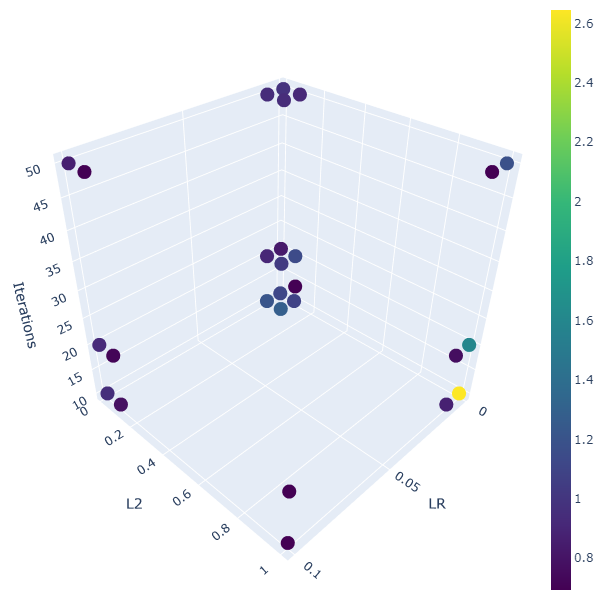
\includegraphics[width=10cm]{../images/3d.png}
\end{center}

As can be seen in the 3D chart above, that represents the resulting losses for each different configuration of parameters (also called hyperparameters space), some values like a very small Learning Rate results in an high loss.\\
What follows are the values for the best configuration

\begin{center}
    \begin{tabular}{ |c|c|c|c| }
        \hline
        Iterations & LR  & L2 & Loss       \\
        \hline
        10         & 0.1 & 1  & 0.69314704 \\
        \hline
    \end{tabular}
    \captionof{table}{TODO}
\end{center}

For the same configuration

\begin{center}
    \begin{tabular}{ |c|c|c|c|c|c|c|c|c| }
        \hline
        TN & TP & FN & FP & Preicision & Recall & F1 & Accuracy & Specificity \\
        \hline
        0  & 0  & 0  & 0  & 0          & 0      & 0  & 0        & 0           \\
        \hline
    \end{tabular}
    \captionof{table}{TODO}
\end{center}

And the following ROC curve

\begin{center}
    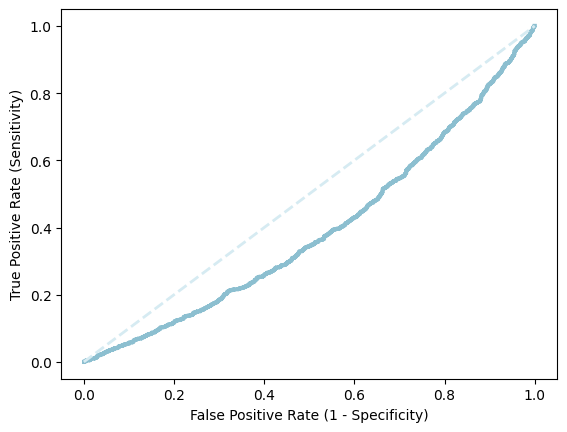
\includegraphics[width=10cm]{../images/parallel_roc.png}
\end{center}

TEMPI

\subsection{Mini Batch}

Another technique described before is the use of Mini Batches, chunk of the train datasets after each one the parameters are updated that should result in a better convergence rate.\\
However OCNTINUARE

\begin{center}
    \begin{tabular}{ |c|c|c|c|c|c|c|c|c| }
        \hline
        TN & TP & FN & FP & Preicision & Recall & F1 & Accuracy & Specificity \\
        \hline
        0  & 0  & 0  & 0  & 0          & 0      & 0  & 0        & 0           \\
        \hline
    \end{tabular}
    \captionof{table}{TODO}
\end{center}

The performances of the parallel enviroment were greatly penalized by this different management of the datasets, resulting in processing time increased by a factor of 10.\\
This can be reconducted on the overhead added by the exchange of messages, that increases with the fragmentation of the memory and computations.

TEMPI

conclusioni

\subsection{Sequential Implementation}

Since the Pyspark implementation is full of options and various optimizations, it's difficult to compare it in term of speed with the proposed implementation.\\
Thus, a sequential version with the same algorithm has been implemented. The difference is not functional but just technical, since the computation is entirely done by numpy and not also by PySpark MapReduce


Time comparison

\subsection{Pyspark ML Logistic Regression}

cose

\begin{center}
    \begin{tabular}{ |c|c|c|c|c|c|c|c|c|c| }
        \hline
        Loss & TN & TP & FN & FP & Preicision & Recall & F1 & Accuracy & Specificity \\
        \hline
        0    & 0  & 0  & 0  & 0  & 0          & 0      & 0  & 0        & 0           \\
        \hline
    \end{tabular}
    \captionof{table}{TODO}
\end{center}

And the following ROC curve

\begin{center}
    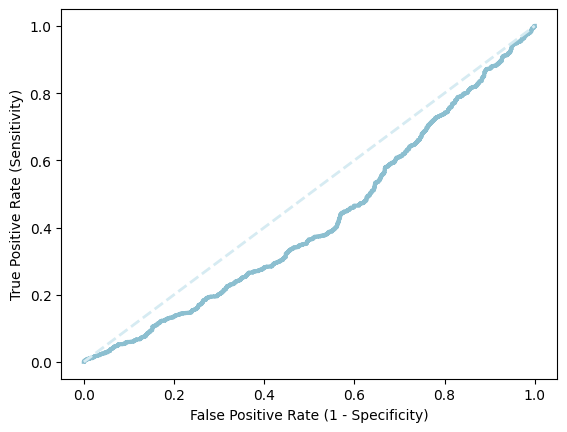
\includegraphics[width=10cm]{../images/ml_logistic.png}
\end{center}

To compare the quality of the custom trained model and the Pyspark model, weights value can be compared. The following table shows the values of each element of the weights for each model and their absolute difference

\begin{center}
    \begin{tabular}{ |c|c|c|c|c|c|c|c|c|c| }
        \hline
        Custom & Pyspark & Absolute difference \\
        \hline
        0      & 0       & 0                   \\
        0      & 0       & 0                   \\
        0      & 0       & 0                   \\
        0      & 0       & 0                   \\
        0      & 0       & 0                   \\
        0      & 0       & 0                   \\
        0      & 0       & 0                   \\
        \hline
    \end{tabular}
    \captionof{table}{TODO}
\end{center}

This comparison can also be easily done in the code using the \textbf{np.allclose}, that compares two vectors elementwise.
As can be seen the elements are close by INSERIRE VALORE, a very small value that implies for the same evaluation algorithm.\\

It's worth notice the weights absolute values are very small, meaning that for both the implementations, none of the corresponding features are impactful on the prediction.\\
It's then clear that the Logistic Regression is not the correct choice for this complex problem.

\subsection{Pyspark ML Decision Tree}

For the same configuration

\begin{center}
    \begin{tabular}{ |c|c|c|c|c|c|c|c|c|c| }
        \hline
        Loss & TN & TP & FN & FP & Preicision & Recall & F1 & Accuracy & Specificity \\
        \hline
        0    & 0  & 0  & 0  & 0  & 0          & 0      & 0  & 0        & 0           \\
        \hline
    \end{tabular}
    \captionof{table}{TODO}
\end{center}

And the following ROC curve

\begin{center}
    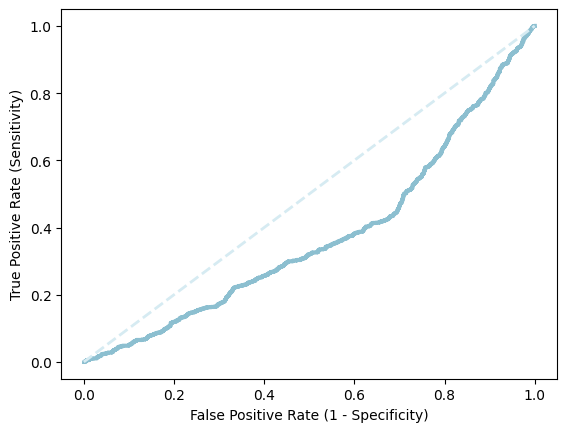
\includegraphics[width=10cm]{../images/tree_roc.png}
\end{center}

\section{Diverted Flights}

%----------------------------------------------------------------------------------------
%	RESULTS AND CONCLUSIONS
%----------------------------------------------------------------------------------------

\section{Results and Conclusions}

The reason of this experiments was to reproduce a complete flow to create and train a Logistic Regression model to classify flights data.\\
The dataset preprocessing has been successfully parallelized using PySpark, but the lack of a proper distributed system to test on lead to worse performances compared to the pandas implementation.\\
It's still important to notice that the parallelization overhead was strangely high even on a single worker configuration, leading to think part of it is by default in PySpark.\\

Instead, the model built using SGD, L2 Regularization, Normalization and Batching (properly tuned) resulted in an accuracy similar to the state-of-art Sklearn implementation.\\
Both of the models probably converged to a local minimum, that would explain the high loss, and this could be explained by the Logistic Regression being a weak model for a real world complex problem like the one taken in consideration.

%----------------------------------------------------------------------------------------
%	BIBLIOGRAPHY
%----------------------------------------------------------------------------------------

\printbibliography % Output the bibliography

% Logistic Regression
% Spark/PySpark
% Kaggle Dataset
% Mini Batch
% L2 Regularization
% Normalization
% SGD
% Il solver di Sklearn
% sklearn, numpy, pandas
% binary cross entropy
% sigmoid

%----------------------------------------------------------------------------------------

\end{document}

% todo

% DEFINIZIONI
% ESPERIMENTI PREPROCESSING
% Performances del modello
% Add Bold words
% README
